\documentclass[12pt,fleqn]{exam}
\usepackage{pifont,bbding,url}
\usepackage{dingbat}
\usepackage{amsmath}
\usepackage{fleqn}
\usepackage{epsfig}
\usepackage{pdfpages}
\usepackage{mathptm}
\usepackage[activate={true,nocompatibility},final,tracking=true,kerning=true,spacing=true,factor=1100,stretch=10,shrink=10]{microtype}
\usepackage{color}
\usepackage{enumerate}
%\usepackage[euler-digits,euler-hat-accent,T1]{eulervm}
\usepackage{amssymb, wasysym, enumerate}
\shadedsolutions
%\definecolor{SolutionColor}{rgb}{0.9,1,1}
\definecolor{SolutionColor}{rgb}{1,1,0.7}
\addpoints
\boxedpoints
\pointsinmargin
\pointname{pts}

\newcommand{\dotprod}{\, {\scriptzcriptztyle \stackrel{\bullet}{{}}}\,}
\begin{document}

\newcommand{\reals}{\mathbf{R}}
\newcommand{\bi}{\mathbf{i}}
\newcommand{\bj}{\mathbf{j}}
\newcommand{\bk}{mathbf{k}}

\newcommand{\euler}{\mathrm{e}}
\newcommand{\ex}{1}
\newenvironment{alphalist}{
  \begin{enumerate}[(a)]
    \addtolength{\itemsep}{-1.0\itemsep}}
  {\end{enumerate}}

\newenvironment{handlist}{
  \begin{enumerate}[\leftthumbsup]
    \addtolength{\itemsep}{-1.0\itemsep}}
  {\end{enumerate}}

\large
\vspace{0.1in}
\noindent\makebox[3.0truein][l]{{\bf MATH 202}}
{\bf Name:}\hrulefill\
\noindent \makebox[3.0truein][l]{\bf In class work 7}
{\bf Row:}\hrulefill\

“If money can fix it, it’s not a problem.”  \hfill  {Tom (or Ray) Magliozzi}
\normalsize



\begin{questions}


\question [5] Find the work done moving a $42$ kg mass from $x= -2 $ to $x =5$ if the position dependent force is $F(x)= \begin{cases} x & x < 1 \\ 1-x & x \geq1 \end{cases} \), where
the units of force are Newtons and the units of distance are meters.
\begin{solution}[3.0in] 
\begin{align*}
\mbox{work} = \frac{5}{2}.
\end{align*}
\end{solution}

\question[5]  Find the \emph{numerical   value} of  \(\displaystyle  \int_3^8 \frac{1}{8 - 3 x} \mathrm{d} x \).   
\begin{solution}[3.0in]
\[
 \int_3^8 \frac{1}{10 - 5 x} \, \mathrm{d} x  = \frac{\ln{(5)}}{5}-\frac{\ln{(30)}}{5}.
\]
\end{solution}


\question[5] Find a general solution to the DE \(\displaystyle -y \frac{\mathrm{d} y}{\mathrm{d} x} = x  \).

\begin{solution}%[2.5in]
 \[ \frac{1}{2} y^2 =  \frac{1}{2} x^2  + c,\]
 where $c \in \reals$.
\end{solution}

%\newpage


\question Find a formula for each derivative:
\begin{parts}

\part[5]  \(\displaystyle \frac{\mathrm{d}}{\mathrm{d} x} \left( x \mathrm{e}^{1/x^2}  \right) \) 
\begin{solution}[1.15in]
  \begin{equation*}
    2 x^2 \mathrm{e}^{x^2}+\mathrm{e}^{x^2}
  \end{equation*}

\end{solution}

\part[5]  \(\displaystyle \frac{\mathrm{d}}{\mathrm{d} x} \left(\frac{\exp(x) - \exp(-x)}{2} \right) \) 
\begin{solution}[1.15in]
\begin{equation*}
  \frac{\exp(x) - \exp(-x)}{2}
\end{equation*}
\end{solution}
\part[5]  \(\displaystyle \frac{\mathrm{d}}{\mathrm{d} x} \left( x  \euler^x \right) \) 
\begin{solution}[1.15in]
\[
1 + \ln(x).
\]
\end{solution}

\part   \(\displaystyle \frac{\mathrm{d}}{\mathrm{d} x}  \ln \left(\frac{1+x}{1-x}\right)$

\begin{solution}[1.15in]
\[
\-\frac{2}{{1-{x}^{2}}}.
\]
\end{solution}


\end{parts}

\question [5] Find the numerical value of $\int_{1}^2 x \euler^x + \euler^x  \, \mathrm{d} x$.  \textbf{Hint:} Look at your answer to part `c' of the previous question.
\begin{solution}[2.25in]
\[2 \log{(2)}\].
\end{solution}
%\newpage

\question Let \(Q\) be the portion of the \(x y\) plane described by \(0 \leq x \leq 1 \) and \(0  \leq y \leq 1 - |x| \).


\begin{parts}

\part [5] Draw a nicely \emph{labeled} picture of the set \(Q\).

\begin{solution}[2.5in] 

\centering
%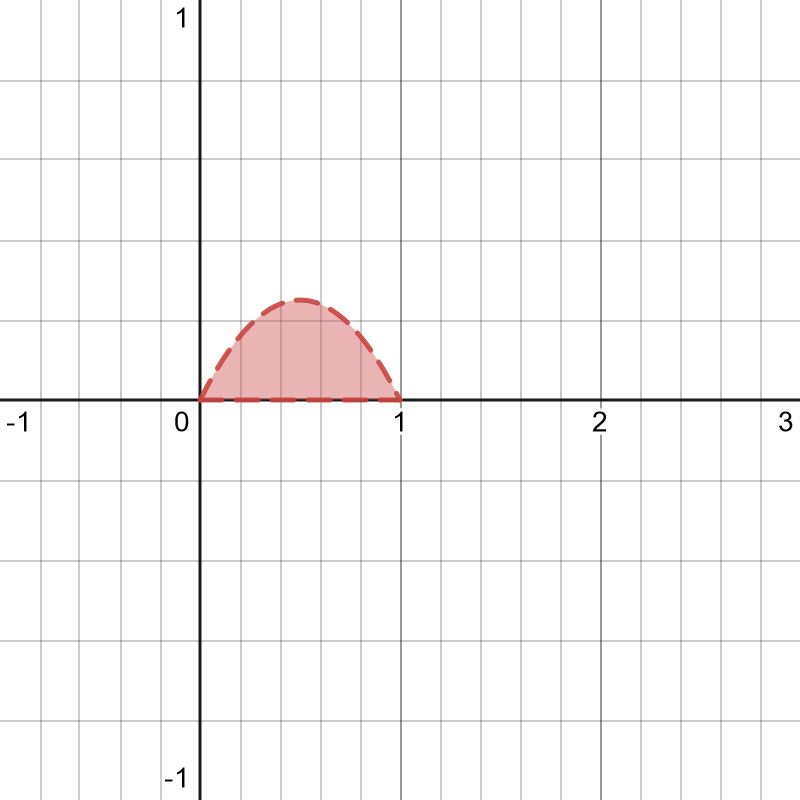
\includegraphics[scale=0.25]{desmos-graph(55)}

\end{solution}

%\newpage

\part [5] Using \emph{disks} (that is strips \emph{perpendicular} to the axis of rotation), find the \emph{volume}
of the solid generated by rotating \(Q\) about the \(x\) axis. Express the result as a \emph{definite integral}, but
\textbf{do not} find the numerical value of the definite integral.

\begin{solution}[2.5in] 
\[
   \pi \int_0^1  x^2 (1-x)^2  \, \mathrm{d} x.
\]
\end{solution}

%\newpage
\part [5] Using \emph{shells} (that is, strips \emph{parallel} to the axis of rotation), find the \emph{volume}
of the solid generated by rotating \(Q\) about the \(x\) axis. Express the result as a \emph{definite integral}, but
\textbf{do not} find the numerical value of the definite integral.


\begin{solution}[2.5in] 
\[
   2 \pi \int_0^{1/4}  y  \sqrt{1-4 y}  \, \mathrm{d} y.
\]
\end{solution}

\part [5] Using a strip that is parallel to the $y$ axis, find area of $Q$.

\begin{solution}[2.5in] 
  \begin{equation}
   \frac{1}{6}.
  \end{equation}

\end{solution}

\part [5] Using a strip that is parallel to the $y$ axis, find the $y$ coordinate of the centroid of $Q$.

\begin{solution}[2.5in] 
  \begin{equation}
    \frac{1}{10}.
   \end{equation}
\end{solution}

\part [5] Using a strip that is parallel to the $y$ axis, find the $x$ coordinate of the centroid of $Q$.

\begin{solution}[2.5in] 

  \begin{equation}
    \frac{1}{2}.
   \end{equation}
\end{solution}
\end{parts}

\question[5] Express the arclength of the portion of the ellipse $x^2 +  8 y^2 = 1$ with $y \leq 0$ and endpoints 
$(x=-1, y=0)$ and $(x=1, y = 0)$. Do not
attempt to find the numerical value of the definite integral.
\begin{solution}[2.5in]
\[\int_{2}^{3}{\left. \sqrt{\frac{2 {{x}^{2}}-1}{{{x}^{2}}-1}} \, \mathrm{d} x\right.}.\]
\end{solution}



\end{questions}
%\includepdf[pages={1-}]{cheat_sheet.pdf}     
\end{document}